\PassOptionsToPackage{unicode=true}{hyperref} % options for packages loaded elsewhere
\PassOptionsToPackage{hyphens}{url}
%
\documentclass[14 pt,ignorenonframetext,]{beamer}
\usepackage{pgfpages}
\setbeamertemplate{caption}[numbered]
\setbeamertemplate{caption label separator}{: }
\setbeamercolor{caption name}{fg=normal text.fg}
\beamertemplatenavigationsymbolsempty
% Prevent slide breaks in the middle of a paragraph:
\widowpenalties 1 10000
\raggedbottom
\setbeamertemplate{part page}{
\centering
\begin{beamercolorbox}[sep=16pt,center]{part title}
  \usebeamerfont{part title}\insertpart\par
\end{beamercolorbox}
}
\setbeamertemplate{section page}{
\centering
\begin{beamercolorbox}[sep=12pt,center]{part title}
  \usebeamerfont{section title}\insertsection\par
\end{beamercolorbox}
}
\setbeamertemplate{subsection page}{
\centering
\begin{beamercolorbox}[sep=8pt,center]{part title}
  \usebeamerfont{subsection title}\insertsubsection\par
\end{beamercolorbox}
}
\AtBeginPart{
  \frame{\partpage}
}
\AtBeginSection{
  \ifbibliography
  \else
    \frame{\sectionpage}
  \fi
}
\AtBeginSubsection{
  \frame{\subsectionpage}
}
\usepackage{lmodern}
\usepackage{amssymb,amsmath}
\usepackage{ifxetex,ifluatex}
\usepackage{fixltx2e} % provides \textsubscript
\ifnum 0\ifxetex 1\fi\ifluatex 1\fi=0 % if pdftex
  \usepackage[T1]{fontenc}
  \usepackage[utf8]{inputenc}
  \usepackage{textcomp} % provides euro and other symbols
\else % if luatex or xelatex
  \usepackage{unicode-math}
  \defaultfontfeatures{Ligatures=TeX,Scale=MatchLowercase}
\fi
% use upquote if available, for straight quotes in verbatim environments
\IfFileExists{upquote.sty}{\usepackage{upquote}}{}
% use microtype if available
\IfFileExists{microtype.sty}{%
\usepackage[]{microtype}
\UseMicrotypeSet[protrusion]{basicmath} % disable protrusion for tt fonts
}{}
\IfFileExists{parskip.sty}{%
\usepackage{parskip}
}{% else
\setlength{\parindent}{0pt}
\setlength{\parskip}{6pt plus 2pt minus 1pt}
}
\usepackage{hyperref}
\hypersetup{
            pdftitle={Generalized Additive Model (GAM)},
            pdfauthor={Hsiao-Hang \& Oscar},
            pdfborder={0 0 0},
            breaklinks=true}
\urlstyle{same}  % don't use monospace font for urls
\newif\ifbibliography
\usepackage{color}
\usepackage{fancyvrb}
\newcommand{\VerbBar}{|}
\newcommand{\VERB}{\Verb[commandchars=\\\{\}]}
\DefineVerbatimEnvironment{Highlighting}{Verbatim}{commandchars=\\\{\}}
% Add ',fontsize=\small' for more characters per line
\newenvironment{Shaded}{}{}
\newcommand{\AlertTok}[1]{\textcolor[rgb]{1.00,0.00,0.00}{\textbf{#1}}}
\newcommand{\AnnotationTok}[1]{\textcolor[rgb]{0.38,0.63,0.69}{\textbf{\textit{#1}}}}
\newcommand{\AttributeTok}[1]{\textcolor[rgb]{0.49,0.56,0.16}{#1}}
\newcommand{\BaseNTok}[1]{\textcolor[rgb]{0.25,0.63,0.44}{#1}}
\newcommand{\BuiltInTok}[1]{#1}
\newcommand{\CharTok}[1]{\textcolor[rgb]{0.25,0.44,0.63}{#1}}
\newcommand{\CommentTok}[1]{\textcolor[rgb]{0.38,0.63,0.69}{\textit{#1}}}
\newcommand{\CommentVarTok}[1]{\textcolor[rgb]{0.38,0.63,0.69}{\textbf{\textit{#1}}}}
\newcommand{\ConstantTok}[1]{\textcolor[rgb]{0.53,0.00,0.00}{#1}}
\newcommand{\ControlFlowTok}[1]{\textcolor[rgb]{0.00,0.44,0.13}{\textbf{#1}}}
\newcommand{\DataTypeTok}[1]{\textcolor[rgb]{0.56,0.13,0.00}{#1}}
\newcommand{\DecValTok}[1]{\textcolor[rgb]{0.25,0.63,0.44}{#1}}
\newcommand{\DocumentationTok}[1]{\textcolor[rgb]{0.73,0.13,0.13}{\textit{#1}}}
\newcommand{\ErrorTok}[1]{\textcolor[rgb]{1.00,0.00,0.00}{\textbf{#1}}}
\newcommand{\ExtensionTok}[1]{#1}
\newcommand{\FloatTok}[1]{\textcolor[rgb]{0.25,0.63,0.44}{#1}}
\newcommand{\FunctionTok}[1]{\textcolor[rgb]{0.02,0.16,0.49}{#1}}
\newcommand{\ImportTok}[1]{#1}
\newcommand{\InformationTok}[1]{\textcolor[rgb]{0.38,0.63,0.69}{\textbf{\textit{#1}}}}
\newcommand{\KeywordTok}[1]{\textcolor[rgb]{0.00,0.44,0.13}{\textbf{#1}}}
\newcommand{\NormalTok}[1]{#1}
\newcommand{\OperatorTok}[1]{\textcolor[rgb]{0.40,0.40,0.40}{#1}}
\newcommand{\OtherTok}[1]{\textcolor[rgb]{0.00,0.44,0.13}{#1}}
\newcommand{\PreprocessorTok}[1]{\textcolor[rgb]{0.74,0.48,0.00}{#1}}
\newcommand{\RegionMarkerTok}[1]{#1}
\newcommand{\SpecialCharTok}[1]{\textcolor[rgb]{0.25,0.44,0.63}{#1}}
\newcommand{\SpecialStringTok}[1]{\textcolor[rgb]{0.73,0.40,0.53}{#1}}
\newcommand{\StringTok}[1]{\textcolor[rgb]{0.25,0.44,0.63}{#1}}
\newcommand{\VariableTok}[1]{\textcolor[rgb]{0.10,0.09,0.49}{#1}}
\newcommand{\VerbatimStringTok}[1]{\textcolor[rgb]{0.25,0.44,0.63}{#1}}
\newcommand{\WarningTok}[1]{\textcolor[rgb]{0.38,0.63,0.69}{\textbf{\textit{#1}}}}
\usepackage{graphicx,grffile}
\makeatletter
\def\maxwidth{\ifdim\Gin@nat@width>\linewidth\linewidth\else\Gin@nat@width\fi}
\def\maxheight{\ifdim\Gin@nat@height>\textheight\textheight\else\Gin@nat@height\fi}
\makeatother
% Scale images if necessary, so that they will not overflow the page
% margins by default, and it is still possible to overwrite the defaults
% using explicit options in \includegraphics[width, height, ...]{}
\setkeys{Gin}{width=\maxwidth,height=\maxheight,keepaspectratio}
\setlength{\emergencystretch}{3em}  % prevent overfull lines
\providecommand{\tightlist}{%
  \setlength{\itemsep}{0pt}\setlength{\parskip}{0pt}}
\setcounter{secnumdepth}{0}

% set default figure placement to htbp
\makeatletter
\def\fps@figure{htbp}
\makeatother


\title{Generalized Additive Model (GAM)}
\providecommand{\subtitle}[1]{}
\subtitle{study group}
\author{Hsiao-Hang \& Oscar}
\providecommand{\institute}[1]{}
\institute{Institute of Oceanography, National Taiwan University}
\date{19 December, 2019}

\begin{document}
\frame{\titlepage}

\begin{frame}{General form}
\protect\hypertarget{general-form}{}

\(g(u_i) = X^*_i \theta + f_1(x_{1i}) + f_2(x_{2i}) + f_3(x_{3i}, x_{4i}) + ...\)
(eqn. 3.1)

\begin{itemize}
\tightlist
\item
  GAM specifies the model with \textbf{smooth functions} rather than
  detailed parametric relationships.
\end{itemize}

\end{frame}

\begin{frame}{Univariate smooth functions \(f\)}
\protect\hypertarget{univariate-smooth-functions-f}{}

\(y_i = f(x_i) + \epsilon_i\) (eqn. 3.2)

\(y_i\) : response variable\\
\(f\) : \textbf{smooth function}\\
\(x_i\) : covariate\\
\(\epsilon_i\) : i.i.d. \(N(0, \sigma^2)\) variable (error)\\

\begin{itemize}
\tightlist
\item
  The smooth function can then be expressed as some\\
  \emph{basis functions} \((b)\) with parameter \(\beta\)
\end{itemize}

\(f(x_i) = \sum_{j=1}^{q} b_j(x)\beta_j\)

\end{frame}

\begin{frame}{Simple example of smooth function: 4th order polynomial
basis}
\protect\hypertarget{simple-example-of-smooth-function-4th-order-polynomial-basis}{}

\(f(x) = \beta_1 + x\beta_2 + x^2\beta_3 + x^3\beta_4 + x^4\beta_5\)

\begin{itemize}
\item
  Fig. 3.1 and Fig. 3.2
\item
  Polynomial basis can be problematic\ldots{}\textbf{spline bases} are
  more common
\end{itemize}

\end{frame}

\begin{frame}[fragile]{Cubic spline basis}
\protect\hypertarget{cubic-spline-basis}{}

\begin{itemize}
\item
  Determine a number of \textbf{knots (k)}
\item
  Fit \(y\) with \(k\) cubic functions plus one constant and one 1st
  term
\item
  The cubic function is written in \textbf{eqn 3.4}
\item
  cubic spline function in \emph{R} (\texttt{z} is rank \(q\))
\end{itemize}

\begin{Shaded}
\begin{Highlighting}[]
\NormalTok{rk <-}\StringTok{ }\ControlFlowTok{function}\NormalTok{(x, z) }\CommentTok{# R(x,z) for cubic spline on [0,1] }
\NormalTok{  \{ }
\NormalTok{  ((z}\FloatTok{-0.5}\NormalTok{)}\OperatorTok{^}\DecValTok{2-1}\OperatorTok{/}\DecValTok{12}\NormalTok{) }\OperatorTok{*}\StringTok{ }\NormalTok{((x}\FloatTok{-0.5}\NormalTok{)}\OperatorTok{^}\DecValTok{2-1}\OperatorTok{/}\DecValTok{12}\NormalTok{)}\OperatorTok{/}\DecValTok{4}\OperatorTok{-}\StringTok{ }\NormalTok{((}\KeywordTok{abs}\NormalTok{(x}\OperatorTok{-}\NormalTok{z)}\OperatorTok{-}\FloatTok{0.5}\NormalTok{)}\OperatorTok{^}\DecValTok{4}\OperatorTok{-}\NormalTok{(}\KeywordTok{abs}\NormalTok{(x}\OperatorTok{-}\NormalTok{z)}\OperatorTok{-}\FloatTok{0.5}\NormalTok{)}\OperatorTok{^}\DecValTok{2}\OperatorTok{/}\DecValTok{2}\OperatorTok{+}\DecValTok{7}\OperatorTok{/}\DecValTok{240}\NormalTok{)}\OperatorTok{/}\DecValTok{24}
\NormalTok{\}}
\end{Highlighting}
\end{Shaded}

\end{frame}

\begin{frame}{}
\protect\hypertarget{section}{}

When \(k = 4\), there are 4 cubic functions.\\
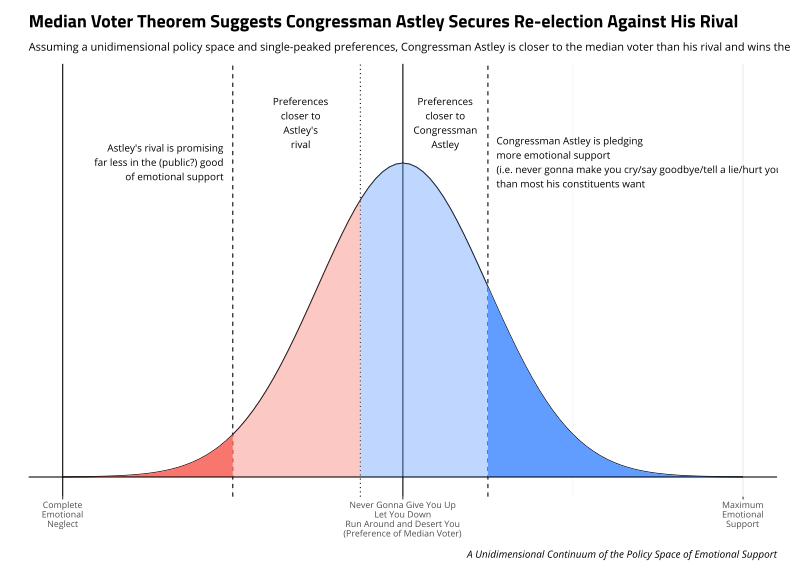
\includegraphics{GAM_01_slidy_files/figure-beamer/unnamed-chunk-2-1.pdf}

\end{frame}

\begin{frame}[fragile]{Example of cubic spline basis}
\protect\hypertarget{example-of-cubic-spline-basis}{}

Data

\begin{Shaded}
\begin{Highlighting}[]
\NormalTok{size <-}\StringTok{ }\KeywordTok{c}\NormalTok{(}\FloatTok{1.42}\NormalTok{,}\FloatTok{1.58}\NormalTok{,}\FloatTok{1.78}\NormalTok{,}\FloatTok{1.99}\NormalTok{,}\FloatTok{1.99}\NormalTok{,}\FloatTok{1.99}\NormalTok{,}\FloatTok{2.13}\NormalTok{,}\FloatTok{2.13}\NormalTok{,}\FloatTok{2.13}\NormalTok{,}\FloatTok{2.32}\NormalTok{,}\FloatTok{2.32}\NormalTok{,}\FloatTok{2.32}\NormalTok{,}\FloatTok{2.32}\NormalTok{,}\FloatTok{2.32}\NormalTok{,}\FloatTok{2.43}\NormalTok{,}\FloatTok{2.43}\NormalTok{,}\FloatTok{2.78}\NormalTok{,}\FloatTok{2.98}\NormalTok{,}\FloatTok{2.98}\NormalTok{)}
\NormalTok{wear <-}\StringTok{ }\KeywordTok{c}\NormalTok{(}\FloatTok{4.0}\NormalTok{,}\FloatTok{4.2}\NormalTok{,}\FloatTok{2.5}\NormalTok{,}\FloatTok{2.6}\NormalTok{,}\FloatTok{2.8}\NormalTok{,}\FloatTok{2.4}\NormalTok{,}\FloatTok{3.2}\NormalTok{,}\FloatTok{2.4}\NormalTok{,}\FloatTok{2.6}\NormalTok{,}\FloatTok{4.8}\NormalTok{,}\FloatTok{2.9}\NormalTok{,}\FloatTok{3.8}\NormalTok{,}\FloatTok{3.0}\NormalTok{,}\FloatTok{2.7}\NormalTok{,}\FloatTok{3.1}\NormalTok{,}\FloatTok{3.3}\NormalTok{,}\FloatTok{3.0}\NormalTok{,}\FloatTok{2.8}\NormalTok{,}\FloatTok{1.7}\NormalTok{)}

\NormalTok{x <-}\StringTok{ }\NormalTok{size }\OperatorTok{-}\StringTok{ }\KeywordTok{min}\NormalTok{(size)}
\NormalTok{x <-}\StringTok{ }\NormalTok{x}\OperatorTok{/}\KeywordTok{max}\NormalTok{(x)}
\end{Highlighting}
\end{Shaded}

Function for generating the model matrix

\begin{Shaded}
\begin{Highlighting}[]
\NormalTok{spl.X <-}\StringTok{ }\ControlFlowTok{function}\NormalTok{(x,xk) }\CommentTok{# set up model matrix for cubic penalized regression spline }
\NormalTok{  \{ q <-}\StringTok{ }\KeywordTok{length}\NormalTok{(xk) }\OperatorTok{+}\StringTok{ }\DecValTok{2} \CommentTok{# number of parameters }
\NormalTok{    n <-}\StringTok{ }\KeywordTok{length}\NormalTok{(x) }\CommentTok{# number of data }
\NormalTok{    X <-}\StringTok{ }\KeywordTok{matrix}\NormalTok{(}\DecValTok{1}\NormalTok{, n, q) }\CommentTok{# initialized model matrix }
\NormalTok{    X[,}\DecValTok{2}\NormalTok{] <-}\StringTok{ }\NormalTok{x  }\CommentTok{# set second column to x}
\NormalTok{    X[,}\DecValTok{3}\OperatorTok{:}\NormalTok{q] <-}\StringTok{ }\KeywordTok{outer}\NormalTok{(x, xk, }\DataTypeTok{FUN =}\NormalTok{ rk) }\CommentTok{# and remaining to R(x,xk) }
\NormalTok{    X}
\NormalTok{\}}
\end{Highlighting}
\end{Shaded}

\end{frame}

\begin{frame}{}
\protect\hypertarget{section-1}{}

Results\ldots{}\\
\includegraphics{GAM_01_slidy_files/figure-beamer/echo-1.pdf}

\end{frame}

\begin{frame}{Knots determine the smoothness}
\protect\hypertarget{knots-determine-the-smoothness}{}

\begin{itemize}
\item
  How many knots?
\item
  \textbf{Penalized regression splines}

  Minimize the
  following\ldots{}\(||y - X\beta|| + \boldsymbol{\lambda \int_{0}^{1}[f''(x)]^2dx}\)\\

  High \(\lambda\) penalizes high wiggliness
  (\(\int_{0}^{1}[f''(x)]^2dx\))

  Fig. 3.8
\item
  Still need to determine a number of knots
\end{itemize}

\end{frame}

\begin{frame}{To determine \(\lambda\)}
\protect\hypertarget{to-determine-lambda}{}

\begin{itemize}
\item
  Ordinary cross validation (OCV)\\
  Leave one data point at a time when doing cross validation
\item
  Generalized cross validation (GCV)\\
  Use \emph{influence matrix} to estimate the deviance when leaving one
  data point out Fig. 3.10
\end{itemize}

\end{frame}

\begin{frame}{Additive model (more than one \(x\))}
\protect\hypertarget{additive-model-more-than-one-x}{}

\(y_i = f_1(x_{1i}) + f_2(x_{2i}) + \epsilon_i\)

All calculations are conceptually the same as mentioned above.

\end{frame}

\begin{frame}{Generalized additive model}
\protect\hypertarget{generalized-additive-model}{}

Due to the link function, penalized likelihood is being maximized.

In practice, \textbf{penalized iteratively re-weighted least square
(P-IRLS)} is implemented.

\end{frame}

\end{document}
